\cotefile{156-7}
\scanpage{73}
\mspage{72}

on a une notion de ``support \unsure{minimal}'' \unsure{subordonné} à cette figure, \unsure{l'ens.|l'ens} \inserted{\unsure{ordonné}} de ses supports s'identifie à $\unsure{\mathcal{P}|\mathscr{P}}(\widetilde F)$. Et si $F'\unsure{\preceq|\leq}F$ est une subdivision, plus gén. $F'\ll F$ un raffinement, on \unsure{sent|sait} comment ``passer'' de l'un à l'autre, via
\[
\unsure{\varphi|\phi}:\widetilde{F'}\longrightarrow\widetilde F
\]
induisant
\[
\varphi^*:\mathcal{P}(\widetilde F)\longrightarrow\mathcal{P}(\widetilde{F'}).
\]

\unsure{Il} ne \unsure{semblerait} pas, dans le cas d'un atlas qui ne soit \unsure{quasi-constructible}, qu'on puisse interpréter \deleted{\unsure{donc}} de façon canonique les $\mathcal{P}(\widetilde F)$, pour des figures \unsure{différentes|differentes} (et qui ne seraient ni compatibles, ni \unsure{reliées|reliés} par $F'\ll F$, ni \inserted{pré-}compatibles dans le sens qu'elles deviennent compatibles après \unsure{subd.|subdiv.} de l'une et de l'autre\ldots), comme des parties d'un même ensemble $\mathcal{P}(P)$ disons, où $P$ est un ensemble de ``points'' associé d'une façon ou d'une autre au \deleted{\unsure{M.}} Atlas $M$.

On va définir cependant la notion de ``réalisation par supports'' d'un \unsure{stratos|Atlas}, dans un ensemble $P$ de ``points''.
\scanpage{74}
\mspage{73}

C'est la donnée d'une application
\[
M\longrightarrow\unsure{\mathcal{P}|\mathscr{P}}(P)\qquad
X\unsure{\mathrel{\vert\!{-}\!\vert}|\longmapsto}|X|
\]
satisfaisant les conditions
\[
X\ll Y\quad\Longrightarrow\quad |X|\subset |Y|
\tag*{$(\mathrm{i})_M$}
\]
\margin{\uline{application croissante} pour $\ll$, $\subset$}
\[
X\unsure{\bowtie|\mathrel{\gtrless}}Y\quad\Longrightarrow\quad
|X|\cap|Y|=\bigcup_{Z\in\widetilde X\cap\widetilde Y}|Z|
\tag*{$(\mathrm{ii})_M$}
\]
\[
X\parallel Y\quad\Longleftrightarrow\quad |X|\cap|Y|=\varnothing
\tag*{\tikz[baseline=(n.base)]{\node[draw,circle,inner sep=1pt](n){$(\mathrm{iii})_M$};}}
\]
\margin{$\longleftarrow$\ \unsure{le fort} de l'axiome est dans l'implication $\Longleftarrow$}
\margin{(NB on a $\Longrightarrow$ par (ii))}
\[
\deleted{\unsure{X}}\quad X\unsure{\preceq|\leq}Y\unsure{,|\ast}\quad\Longrightarrow\quad |X|=|Y|
\tag*{$(\deleted{\unsure{\mathrm{iii}}}\mathrm{iv})_M$}
\]
\[
\unsure{\backslash}\qquad |X|=\bigcup_{Z\in\unsure{\operatorname{omb}|\operatorname{Somb}|\operatorname{Comb}}(X)}|Z|
\tag*{$(\mathrm{v})_M$}
\]
\[
\begin{aligned}
&\inserted{\text{\tikz[baseline=(n.base)]{\node[draw,circle,inner sep=0.7pt](n){a};}\ }\bigcup_{X\in M}|X|=P,\ \text{et}}\\
&\inserted{\text{\tikz[baseline=(n.base)]{\node[draw,circle,inner sep=0.7pt](n){b};}}}\ \text{Si }x,y\in P,\quad\exists X\in M\ \text{avec}\quad x\in|X|,\ y\notin|X|\\
&\hspace{26em}\text{ou l'inverse}
\end{aligned}
\tag*{$(\unsure{?\mathrm{vi}|\mathrm{vi}})_M$}
\]

NB 1) L'axiome (vi) est dans la nature d'une normalisation; il suffit de remplacer $P$ par son quotient par la relation d'équivalence
\[
x\sim y\quad\Longleftrightarrow\quad M_x=M_y
\qquad (\text{où }M_x=\{X\in M\mid x\in|X|\})
\]

\uline{NB} 2) La condition v implique qu'il suffit de connaître $|Z|$ pour $Z\in L$. \deleted{Mais cette \unsure{fonction}} On \uline{définit} les $|X|$ pour $X$ \unsure{général} par (v). Mais la validité des conditions (i) à (iv) \unsure{requiert|revient} des conditions draconiennes sur $|Z|$. La condition \unsure{(iii)|(ii)} p. ex. équivaut à la $=$ condition \inserted{(ou \unsure{(iii')|(ii')})} pour $X,Y\in L$, $+$ la condition At L2. La condition \unsure{(vi)|(iii)} \deleted{\unsure{doit être automatique} \unsure{moyennant} $L3$ \unsure{la condition} $(\unsure{\mathrm{ii}'|\mathrm{iii}'})$: $\unsure{Z\,X}$,} est automatique moyennant At L3 et \unsure{(ii')|(iii')} (partie $\Rightarrow$). La condition (i) tautologique. Je soupçonne que (iv) résulte des autres conditions. Donc, \unsure{ça revient} \unsure{via l'appl.|à l'appl.} \inserted{(moyennant At L2, L3)}
\[
L\longrightarrow\mathcal{P}(P),\qquad
x\mathrel{\vert\!{-}\!\vert}|x|,
\]
\scanpage{75}
\mspage{74}

Conditions
\begin{tabular}{|p{0.92\linewidth}}
\[
\text{Soient }\unsure{x|a},y\in L,\quad\text{alors}\quad
x\parallel y\quad\Longleftrightarrow\quad |x|\cap|y|=\varnothing
\tag*{$(\mathrm{i})_L$}
\]
\[
\begin{aligned}
&\deleted{\text{\unsure{Comme}}}\quad\forall\unsure{\xi|\zeta},\eta\in P,
\ \inserted{\xi\ne\eta},\ \exists\deleted{\unsure{y}}x\in L,\quad\text{avec}\quad
\xi\in|x|,\ \eta\notin|x|\\
&\hspace{27em}\text{ou l'inverse}
\end{aligned}
\tag*{$(\mathrm{ii})_L$}
\]

\end{tabular}

\uline{Exemple}. $P$ est une ficelle topologique, \deleted{\unsure{orientée}} et $M$ est le \unsure{stratos} des \inserted{liens et des} segments (ou sous-ficelles) de ladite, la fonction support $|x|$ \deleted{est} pour les liens étant la fonction évidente.
% slanted
\margin{\uline{NB} Il faut supposer ici pour la validité de (i), que les ``bouts'' de la ficelle soient connexes}

La condition (ii) n'est pas forcément satisfaite (sûrement pas, si les bouts de la ficelle ne \unsure{sont|st} \unsure{réduits} à des points --- s'ils le sont, on a une bonne chance pour (ii) soit valable\ldots)

Dans tous les cas intéressants des \unsure{stratos|Atlas} à ma connaissance, sauf peut être celui \unsure{de l'Atlas|des Atlas} associé à un ens. ordonné (\unsure{toujours} si on veut) donné ad hoc, on a une notion naturelle de supports $|\ |$.

La question qui se pose alors \unsure{est ici|est bien}: Une telle donnée détermine-t-elle $P$ à isomorphisme canonique près --- p. ex. par \unsure{l'existence} d'un iso can. d'ens. ordonnés ou \deleted{application} \inserted{\unsure{anti-isomorphisme}} \unsure{(}
\[
\underset{\text{ens des supports ``abstraits'' de }M}{\Sigma_M}
\simeq\unsure{\mathcal{P}|\mathscr{P}}(P)\quad??
\]
\scanpage{76}
\mspage{75}

Pour toute partie $A$ de $M$, posons
\[
|A|=\bigcup_{X\in A}|X|
\]
% slanted
\margin{\uline{NB} $|\varnothing|=\varnothing$, et si $\mathrm{vi}_M$ \tikz[baseline=(n.base)]{\node[draw,circle,inner sep=0.7pt] (n) {\unsure{a}};} \unsure{vérifié|vérifiée}, $|M|=P$}

Ceci posé, je \deleted{dis} \inserted{voudrais} que pour deux parties $A,B$ de $M$, on ait
\[
\begin{aligned}
\operatorname{supp}A\subset\operatorname{supp}B
&\overset{?}{\Longleftrightarrow}|A|\subset|B|\\
\text{(ou encore }A\subset\operatorname{supp}B\text{)}&
\end{aligned}
\tag*{(*)}
\]
En effet, \deleted{\unsure{on}} \unsure{la première|le premier} \deleted{\unsure{relation}} \inserted{membre} équivaut à
\[
\operatorname{cosupp}B\subset\operatorname{cosupp}A,
\tag*{\unsure{(a)}}
\]
or \deleted{on a} on a, pour $X\in M$
\[
\begin{aligned}
X\in\operatorname{cosupp}A
&\overset{\mathrm{def}}{\Longleftrightarrow}\deleted{\unsure{A}}X\parallel A
\overset{\mathrm{def}}{\Longleftrightarrow}\forall Y\in A,\ X\parallel Y\\
&\overset{\mathrm{iii}_M}{\Longleftrightarrow}\forall Y\in A,\ |X|\cap|Y|=\varnothing
\Longleftrightarrow |X|\cap|A|=\varnothing
\end{aligned}
\]

Donc l'inclusion $\operatorname{supp}A\subset\operatorname{supp}B$, ou encore \unsure{(a)|(*)}, équivaut à
\[
\forall X\in M,\quad |X|\cap|B|=\varnothing\quad\Longrightarrow\quad |X|\cap|A|=\varnothing.
\tag*{($\bullet$)}
\]
et cette \deleted{\unsure{relation}} \inserted{propriété} sur $(A,B)$ est évidemment impliquée par $|A|\subset|B|$. Donc dans (*) on a $\Longleftarrow$. Pour voir $\Longrightarrow$, il revient au $=$ de montrer que \deleted{\unsure{les}} $|A|\not\subset|B|$ implique l'existence de $X\in M$, avec $|X|\cap|B|=\varnothing$ mais $|X|\cap|A|\ne\varnothing$. Ce n'est pas clair en général, et je \unsure{donnerai} \unsure{peut-être|peut être} contre-exemple \unsure{tantôt}. Mais supposons que $B$ soit un support, i.e.\ \deleted{$\unsure{B}$}
\[
B=\operatorname{supp}B,
\]
\scanpage{77}
\mspage{76}

alors le $1^{\mathrm{er}}$ \unsure{mb|mbr.} de (*) \deleted{\unsure{s'écrit}} équivaut à
\[
A\subset B
\]
qui implique bien $|A|\subset|B|$ tautologiquement. Ainsi

\uline{Lemme \unsure{!|1}} Sous la \inserted{seule} condition $(\mathrm{iii}_M)$, si $A$ et $B$ sont des parties de $M$, on a
\diagram{
\begin{tikzcd}[ampersand replacement=\&,column sep=large,row sep=small]
\operatorname{supp}A\subset\operatorname{supp}B
\arrow[d,phantom,"{\unsure{\Vert|\Updownarrow}}" description]
\& |A|\subset|B|\arrow[l,Rightarrow]\\
(A\subset\operatorname{supp}B)\&
\end{tikzcd}
}
et l'implication inverse est vraie si $B$ est un support (i.e.\ $B=\operatorname{supp}B$).

\uline{Corollaire} L'application
\[
\Sigma_M\longrightarrow\unsure{\mathcal{P}|\mathscr{P}}(P)\qquad A\longmapsto|A|
\]
\begin{tabular}{|p{0.88\linewidth}}
est injective, et la relation d'inclusion dans $\Sigma_M$ est induite par la relation d'inclusion dans $\mathcal{P}(P)$
\end{tabular}

Qu'en est-il de l'intersection $\bigwedge_i$ \inserted{$=\bigcap_i$} et du \deleted{la ``réunion''} sup $\bigvee_i$ des supports?

On a
\[
\begin{aligned}
\left|\bigwedge_i A_i\right|&\subset\bigcap_i|A_i|&\text{tautologique}\\
\left|\bigvee_i A_i\right|&\supset\bigcup_i|A_i|&\text{id}
\end{aligned}
\]
mais je doute qu'on ait tjrs égalité. D'autre part, je dis que
\[
|\unsure{c_M|C_M}(A)|\subset\unsure{R|P}\setminus|A|
\]
\scanpage{78}
\mspage{77}

En effet,
\[
\unsure{C_M|c_M}(A)=\{X\in M\mid X\parallel A\}
=\{X\in M\mid |X|\cap|A|=\varnothing
\]
\inserted{i.e.\ $|\overline X|\subset\unsure{R|P}\setminus A$}
donc
\[
|C_M(A)|=\bigcup\overline X\quad\text{pour }X\unsure{\in|\notin}\deleted{A}M\ \unsure{\text{t.q.}|\text{i.e.}}\quad |X|\subset P\setminus A
\]
d'où l'inclusion dite, sans garantie que ce soit tjrs égalité.

On aimerait aussi avoir, pour $A$ partie quelconque de $M$
\[
|A|\overset{?}{=}|\operatorname{supp}A|,
\tag*{(**)}
\]
alors qu'on a a priori (tautologiquement)
\[
|A|\subset|\operatorname{supp}A|
\]
puisque $A\subset\operatorname{supp}A$. \deleted{\unsure{le}} Donc on voudrait
\[
|\operatorname{supp}A|\subset|A|
\]
ce qui serait conséquence de l'implication inverse (hypothétique) de celle du Lemme. La validité de cette implication inverse, pour $\forall A,B$, est d'ailleurs équivalente au cas particulier d'un couple $(\operatorname{supp}A,A)$, i.e.\ à la validité de (**).

Cela fait donc quelques \unsure{perplexités}, \unsure{liées|liés} aux \unsure{mystères} des \deleted{de} $P$-supports.

Tout \inserted{\unsure{ça}} se \unsure{résoud|résout} si on fait l'hypothèse suivante

\uline{Hyp} Soit $A\subset M$, et $x\in P\setminus|A|$. Alors $\exists X\in M$ avec \deleted{$\unsure{X}$} $X\parallel A$ (i.e.\ $|X|\subset P\setminus|A|$) et $x\in|X|$
\scanpage{79}
\mspage{78}

Mais ça signifie ni plus ni moins que
\[
\bigcup_{\substack{X\in M\\X\unsure{\parallel|\notin}A}}|X|=P\setminus|A|
\qquad\inserted{\text{i.e. }X\in\operatorname{cosupp}A}
\]
% slanted; the note is enclosed in an oval and linked to the following line.
\margin{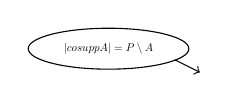
\begin{tikzpicture}[scale=.4,transform shape]
\node at (0,0) {$|\operatorname{cosupp}A|=P\setminus A$};
\draw (0,0) ellipse (2.55 and .65);
\draw[->] (2.1,-.35)--(2.9,-.75);
\end{tikzpicture}}
i.e.\ que l'inclusion $|\unsure{C_M|c_M}(A)|\subset P\setminus|A|$ est une égalité. (En l'occurrence pas seulement pour $A$ $\unsure{\delta|\xi}$ un ensemble support, \unsure{tant} qu'à faire\ldots) Comme $\operatorname{supp}A=\operatorname{cosupp}(\operatorname{cosupp}A)$ on en déduira bien
\[
\begin{aligned}
|\operatorname{supp}A|&=P\setminus(P\setminus|A|)\\
&=A,
\end{aligned}
\]
OK.\ \deleted{$\operatorname{supp}$} Donc

\uline{Lemme 2} Sous les conditions $(\mathrm{iii}_M)$ et $(\mathrm{vi}_M\ \text{a})$, supposons de plus l'hypothèse précédente satisfaite, i.e.
\[
\forall A\subset M,\qquad |\operatorname{cosupp}A|=P\setminus|A|.
\]
Alors pour $\forall A\subset M$, on a
\[
|A|=|\operatorname{supp}A|,
\]
et pour $A,B\subset M$, on a
\diagram{
\begin{tikzcd}[ampersand replacement=\&,column sep=large,row sep=small]
\operatorname{supp}A\subset\operatorname{supp}B
\arrow[r,Leftrightarrow]
\arrow[d,phantom,"{\unsure{\Vert|\Updownarrow}}" description]
\& |A|\subset|B|\\
\bigl(A\subset\operatorname{supp}B
\arrow[d,phantom,"{\Vert}" description]\&\\
\operatorname{cosupp}B\subset\operatorname{cosupp}A\&
\end{tikzcd}
}
\unsure{Cela pour sens|Cela par sens} $\Longleftarrow$ \unsure{connu|comme} dans lemme 1).

L'application (injection, plongement ordonné \inserted{cf Cor. lemme 1})
\[
\Sigma_M\unsure{\mathrel{-}|\longrightarrow}\unsure{\mathcal{P}|\mathscr{P}}(P)
\qquad A\unsure{\mathrel{\vert\!{-}}|\longmapsto}|A|
\]
commute à l'involution $C_M$, $C_P$.
